% !TeX spellcheck = ca
\documentclass{article}
\usepackage[utf8]{inputenc}
\usepackage{amsmath}
\usepackage{ amssymb }
\usepackage{float}
\usepackage{graphicx}

%Tot això hauria d'anar en un pkg, però no sé com és fa
\newcommand*{\assignatura}[1]{\gdef\1assignatura{#1}}
\newcommand*{\grup}[1]{\gdef\3grup{#1}}
\newcommand*{\professorat}[1]{\gdef\4professorat{#1}}
\renewcommand{\title}[1]{\gdef\5title{#1}}
\renewcommand{\author}[1]{\gdef\6author{#1}}
\renewcommand{\date}[1]{\gdef\7date{#1}}
\renewcommand{\baselinestretch}{1.5}
\renewcommand{\maketitle}{ %fa el maketitle de nou
	\begin{titlepage}
		\raggedright{UNIVERSITAT DE LLEIDA \\
			Escola Politècnica Superior \\
			Grau en Enginyeria Informàtica\\
			\1assignatura\\}
		\vspace{5cm}
		\centering\huge{\5title \\}
		\vspace{3cm}
		\large{\6author} \\
		\normalsize{\3grup}
		\vfill
		Professorat : \4professorat \\
		Data : \7date
\end{titlepage}}
%Emplenar a partir d'aquí per a fer el títol : no se com es fa el package
%S'han de renombrar totes, inclús date, si un camp es deixa en blanc no apareix


\title{Complete Sat Report}
\author{Joaquim Picó Mora, Ian Palacín Aliana}
\date{Divendres 28 Maig}
\assignatura{Programació avançada en intel·ligència artificial}
\professorat{Josep Argelich Roma}
\grup{}

\renewcommand{\refname}{Bibliografia}

%Comença el document
\begin{document}
	\maketitle
	\thispagestyle{empty}


%Fer intro?
\section{Introduction}
In this document we explain the most important implementation decisions and problems
encountered during the development of a complete sat solver based on the Davis Putnam
Logemann Loveland algorithm.
%Chachareria per omplir.
%
\section{Skeleton}

The skeleton of the algorithm is that of a DPLL, it is a systematic search using backtracking.
The system used is to propagate the unit clauses until an empty clause  or
dissatisfaction is found. Since there are not always unit clauses available, when
there are no more, a variable is chosen and put in a unit clause, thus continuing the
propagation. \\

The choice of this variable greatly affects the speed of the solver, which is why we have studied
different heuristics that guided the choice. \\

Once the variable is chosen, the recursive function is called twice, once where it is added
to the formula a unitary clause with the positive variable, and one where it is added to the formula
a unit clause with the negative variable. It is in this fork where recursion and backtracking occurs
, because if a solution is found it will be propagated backwards, and in case of
not finding it will follow through the other branches.

%
\section{Heuristics}
In this section we're going to pass trough all the heuristics explaining how had been implemented and also we're going to discuss the results that they have given to us. 
\subsection{Most Ocurrences}
Firstly we have the most ocurrences heuristic. As the name says, the literal that we pick to propagate is the one that apears the most in the formula. In order to get it, we iterate through the clauses and literals adding all the ocurrences of each literal and latter geting the one that appears the most.
\subsection{Most Ocurrences in Minimum Size}
This heuristic gets the literal that appears the most in a minimum clause size. After unit propagation, the minimum size a clause can have is 2 literals, so most of the time we will start with size 2. Another thing to consider is that if there is a tie between two literals or more, we have to break the tie looking for the appearances of those literals in the clauses with one literal more, and if there is another tie with some of them, we have to look for one more...\\
In order to do this, we get the minimum size of the clauses in the formula after the unit propagation and then we get the clauses with that size. After that we count the appearances of the litterals in the clauses get the one the appeared the most. In case of having a tie, we have a function called tiebraker that repeats the same for bigger clauses until it gets the final literal.
\subsection{Most Equilibrated}
This one takes into account the appearances of the literal and the negated literal, counting the times that appear each one of them. After geting the result, it multiplies the appearances of the literal and the appearances of the negated literal and gets the one that results with the biggest number. This means that is the most equilibrated and is the one that we have to chose to propagate.\\
In order to implement it, we used the same strategy that in the most ocurrences heuristic, but this time  instead of counting each literal separetly we count each symbol getting the times that appear positive and negated.
\subsection{Jeroslow Wang}
%
Jeroslow Wang take into account all the occurrences of the literals in the formula, making the appearances of literals in small clauses have more importance due to the formula  $\sum 2^{-len(c)}$. We can see that the smaller is the length of the clause, the better.
In order to do it we iterate through the formula and we make the summation of the occurences of all the literals. The one that results with the bigest value is the one that we pick. 
\subsection{Jeroslow Wang Two Sided}
%
This is an interesting implementation of Jeroslow Wang that we find that takes into the summation of each literal takes into acount the negated literal too. It's implemented the same way as normal Jeroslow Wang, but acounting all the apparences of a symbol.
\subsection{Results}
% Gràfics% Comentar resultats
The graphic that we provide next has been made with the results of executing each heuristic with random 3 cnfs formulas of 75 variables and with a variable number of clauses (X axis). Each formula have been executed 25 times per heuristic and we made the mean in order to get the resulting value of time (Y axis).   
\begin{figure}[H]
  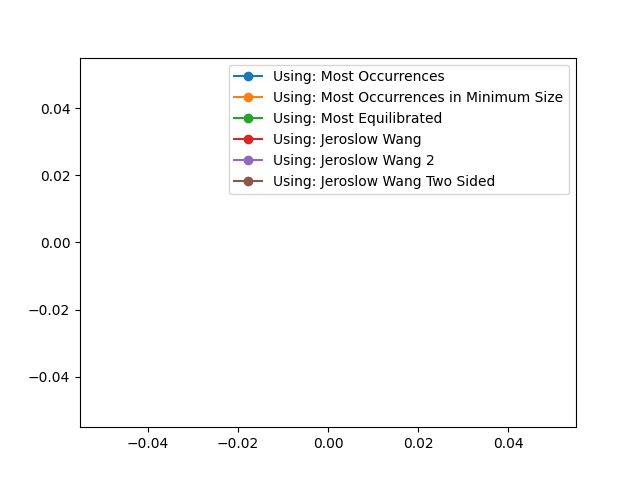
\includegraphics[width=\linewidth]{../utils/plots/heuristics.png}
  \caption{Heuristics comparation.}
  \label{fig:heu}
\end{figure}
In this plot \ref{fig:heu} we can see that the fastest heuristic is the 2 sided Jeroslow Wang. Surprisingly it performs really well, even Jeroslow Wang is not one of the best heuristics as we can see in the plot, it doesn't take care of the same symblol negated literals. Contempling this literals into Jeroslow Wang does not add more complexity in time and as we can see it makes it perform the way better.
The worst heuristic but not for that much is most occurences, which makes sense but is probably the least informed one. 
From the rest, we can see that more or less perform the same way but we can highlight that MOMS heuristic seems to perform better with hard formulas and don't have huge peaks at all.
\section{Python improvements}
In order to make faster python we followed some guides and tested various things:
\begin{itemize}
	\item We found out that maps and list comprehensions are faster than normal for loops, so we used
	them when possible
	\item Python function overhead is notable, so we reduced the number of functions in the critical
	parts of the algorithm. Separating the most executed part of the algorithm in different functions 
	would lead from hundred of thousands to milions extra calls (for real, we checked it with the
	profiler).
	\item We are not big fans of global variables, even less if we are speaking about performance. Local
	variables are much faster.
\end{itemize} 
%
\section{Profiling}
%
As we wanted to optimize the sat, we profiled it using cProfile in order to know wich of the functions were the ones that the algorithm executes the most and the ones in wich spends most of the time. Doing this has hepled us to optimize and improve the code in the critical points.
\section{Conclusions}
During the implementation we came to the conclusion that the best optimizations come from the algorithm
itself, a good heuristic is the angular stone to cut times. 
Once the algorithm is the desired is the time to optimize the code, not before.

We also learned that heuristics are that, heuristic. They shall be treated with caution, as one could
go flawless for some types of problems, but horrendous for others. In fact, we already knew that, nonetheless
we made the mistake several times.
%Chachareria per omplir
\end{document}